\section*{1. Gliederung}
\label{sec:1-gliederung}

\begin{frame}
\frametitle{\begin{center} \Large\bf \nameref{sec:1-gliederung}\end{center}}\vspace{-0.4cm}
    \begin{itemize}
		\item Motivation
		\item Vorwissen
		\item Implementierung, Hardware, Software
		\item Architektur
		\item Latenter Raum
		\item Fazit, Wie kann es weiter gehen
	\end{itemize}
    \vspace{1.0cm}
\end{frame}

\section*{2. Motivation}
\label{sec:2-motivation}

\begin{frame}
\frametitle{\begin{center} \Large\bf \nameref{sec:2-motivation}\end{center}}\vspace{-0.4cm}
    \begin{itemize}
		\item Trial-and-Error Multi-Task Architekturen
		\item Multi-Task Taxonomie
		\item Latente Informationen einzelner Schichten in Single-Task Modellen
		\item Latenten Raum eines Variational Autoencoders verstehen
	\end{itemize}
    \vspace{1.0cm}
\end{frame}

\section*{3. Autoencoder}
\label{sec:3-Autoencoder}

\begin{frame}
\frametitle{\begin{center} \Large\bf \nameref{sec:3-Autoencoder}\end{center}}\vspace{-0.4cm}
    \begin{figure}
		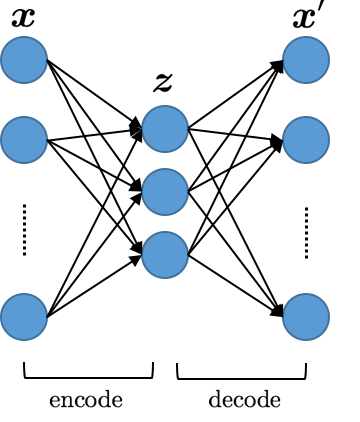
\includegraphics[width=0.6\textwidth]{images/figures/presentation/autoencoder.png}
		\vspace*{15pt}\hbox{\scriptsize Credit:\thinspace{\small\itshape GRID INC}}
	\end{figure}
    \vspace{1.0cm}
\end{frame}

\section*{4. Variational Autoencoder}
\label{sec:4-VAE}

\begin{frame}
\frametitle{\begin{center} \Large\bf \nameref{sec:4-VAE}\end{center}}\vspace{-0.4cm}
    \begin{figure}
		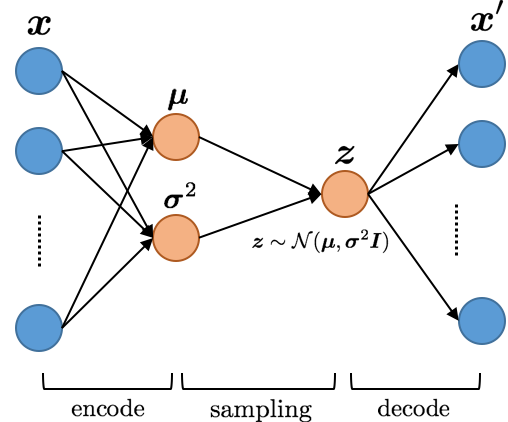
\includegraphics[width=0.7\textwidth]{images/figures/presentation/variational_autoencoder.png}
		\vspace*{15pt}\hbox{\scriptsize Credit:\thinspace{\small\itshape GRID INC}}
	\end{figure}
    \vspace{1.0cm}
\end{frame}


\section*{5. Implementierung, Hardware, Software}
\label{sec:5-impl}

\begin{frame}
\frametitle{\begin{center} \Large\bf \nameref{sec:5-impl}\end{center}}\vspace{-0.4cm}
    \begin{itemize}
		\item Python
		\item Tensorflow
		\item Container der Uni Hannover
		\item Machine-Learning Rechner der UniBw
	\end{itemize}
    \vspace{1.0cm}
\end{frame} 

\section*{6. Architektur Experimente}
\label{sec:6-archExp}
\begin{frame}
\frametitle{\begin{center} \Large\bf \nameref{sec:6-archExp}\end{center}}\vspace{-0.4cm}
    \begin{itemize}
		\item Anzahl von convolutional Schichten
		\item Anzahl von Filtern
		\item Kernel Größe
		\item Max/Average Pooling
	\end{itemize}
    \vspace{1.0cm}
\end{frame} 


\section*{7. Ergebnisse: Schichtanzahl}
\label{sec:7-schichtenzahl}
\begin{frame}
\frametitle{\begin{center} \Large\bf \nameref{sec:7-schichtenzahl}\end{center}}\vspace{-0.4cm}
    \begin{figure}
		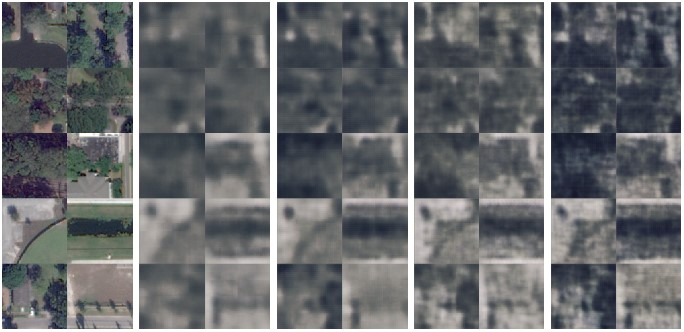
\includegraphics[width=\textwidth]{images/figures/presentation/bad_reconstructions.jpg}
	\end{figure}
    \vspace{1.0cm}
\end{frame} 


\section*{8. Beste Architektur}
\label{sec:8-bestArchitecture}
\begin{frame}
\frametitle{\begin{center} \Large\bf \nameref{sec:8-bestArchitecture}\end{center}}\vspace{-0.4cm}
    \begin{figure}
		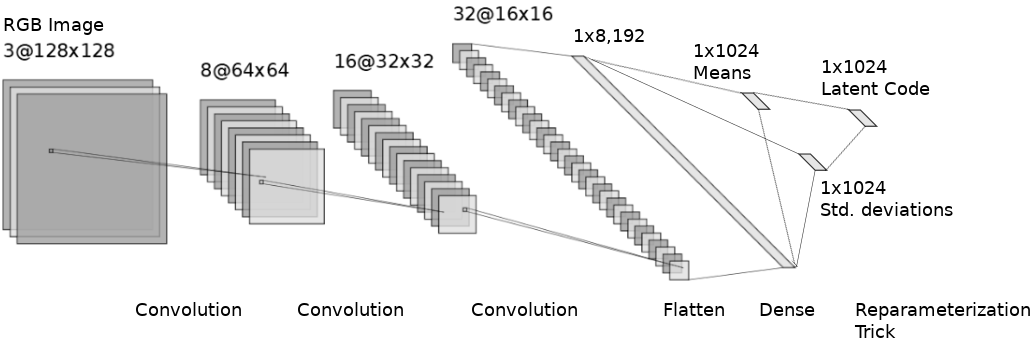
\includegraphics[width=\textwidth]{images/figures/encoder_neural_network.png}
		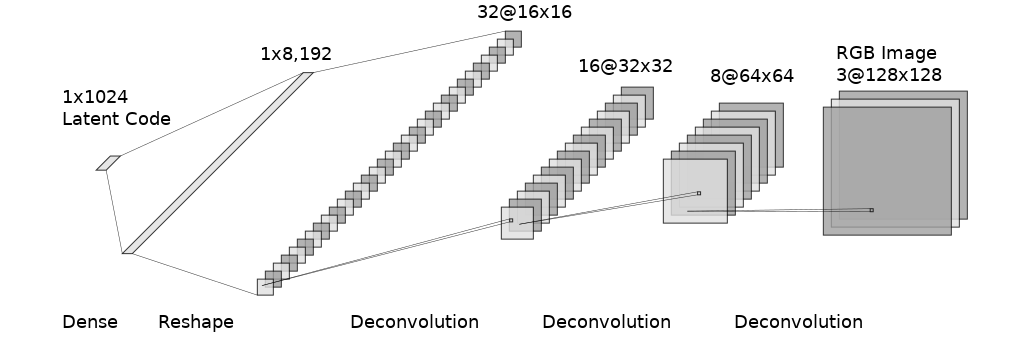
\includegraphics[width=\textwidth]{images/figures/decoder_neural_network.png}
	\end{figure}
    \vspace{1.0cm}
\end{frame} 

\section*{9. Pooling Architektur}
\label{sec:9-poolingArchitecture}
\begin{frame}
\frametitle{\begin{center} \Large\bf \nameref{sec:9-poolingArchitecture}\end{center}}\vspace{-0.4cm}
    \begin{figure}
		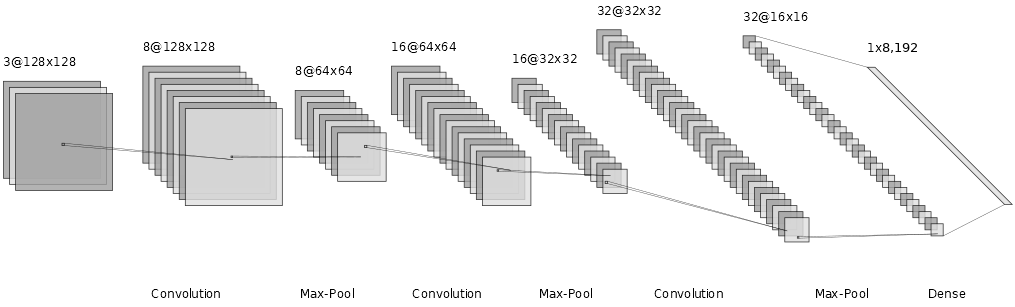
\includegraphics[width=\textwidth]{images/figures/encoder_pooling.png}
	\end{figure}
    \vspace{1.0cm}
\end{frame} 


\section*{10. Training mit 178.000 Bildern}
\label{sec:10-train_with_all}
\begin{frame}
\frametitle{\begin{center} \Large\bf \nameref{sec:10-train_with_all}\end{center}}\vspace{-0.4cm}
    \begin{figure}
		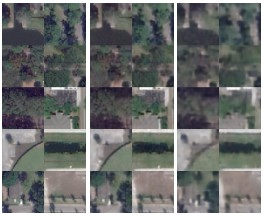
\includegraphics[width=0.8\textwidth]{images/figures/presentation/good_reconstructions.jpg}
	\end{figure}
    \vspace{1.0cm}
\end{frame} 


\section*{11. Latenter Raum Experimente}
\label{sec:11-latentSpaceExperiments}
\begin{frame}
\frametitle{\begin{center} \Large\bf \nameref{sec:11-latentSpaceExperiments}\end{center}}\vspace{-0.4cm}
    \begin{itemize}
		\item 4000 Bilder $=>$ 4000 Encodings
		\item Dimension reduzieren
		\item Visualisieren
	\end{itemize}
    \vspace{1.0cm}
\end{frame} 



\section*{12. t-Stochastic-Neighbor-Embedding}
\label{sec:12-tSNE}
\begin{frame}
\frametitle{\begin{center} \Large\bf \nameref{sec:12-tSNE}\end{center}}\vspace{-0.4cm}
    \begin{itemize}
		\item Machine-Learning Verfahren zur Dimensions Reduktion
		\item Besonders gut geeignet für einzelne Visualisierungen
		\item Fokus auf Kontext von Punkten zu ihren Nachbarn
	\end{itemize}
    \vspace{1.0cm}
\end{frame} 


\section*{13. Ergebnisse: Topographische Klassen}
\label{sec:13-resultsClasses}
\begin{frame}
\frametitle{\begin{center} \Large\bf \nameref{sec:13-resultsClasses}\end{center}}\vspace{-0.4cm}
    \begin{figure}
		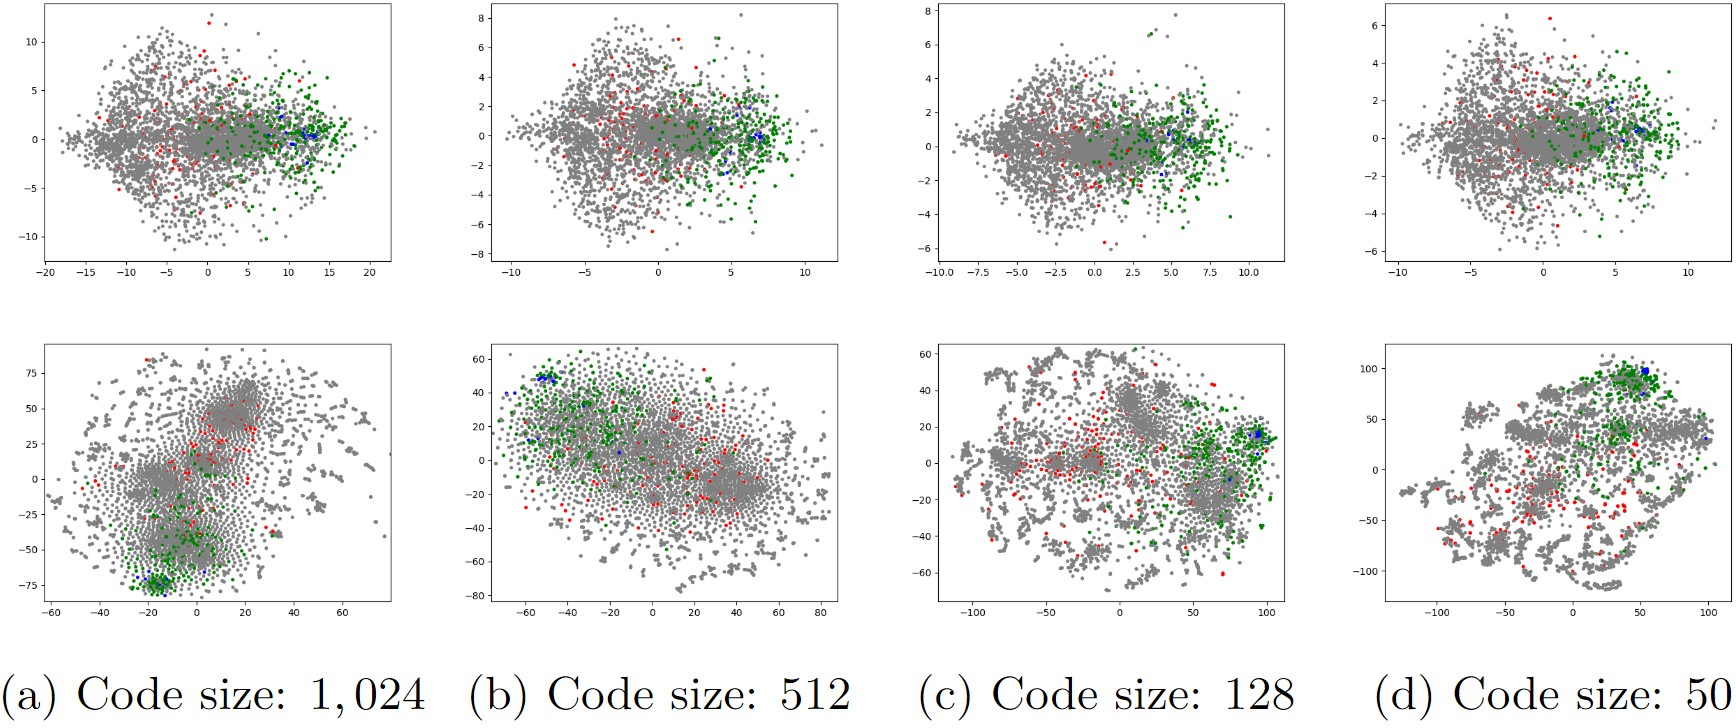
\includegraphics[width=\textwidth]{images/figures/presentation/tsne-Classes.jpg}
	\end{figure}
    \vspace{1.0cm}
\end{frame} 


\section*{14. Ergebnisse: Höhen Daten}
\label{sec:14-heights}
\begin{frame}
\frametitle{\begin{center} \Large\bf \nameref{sec:14-heights}\end{center}}\vspace{-0.4cm}
    \begin{figure}
		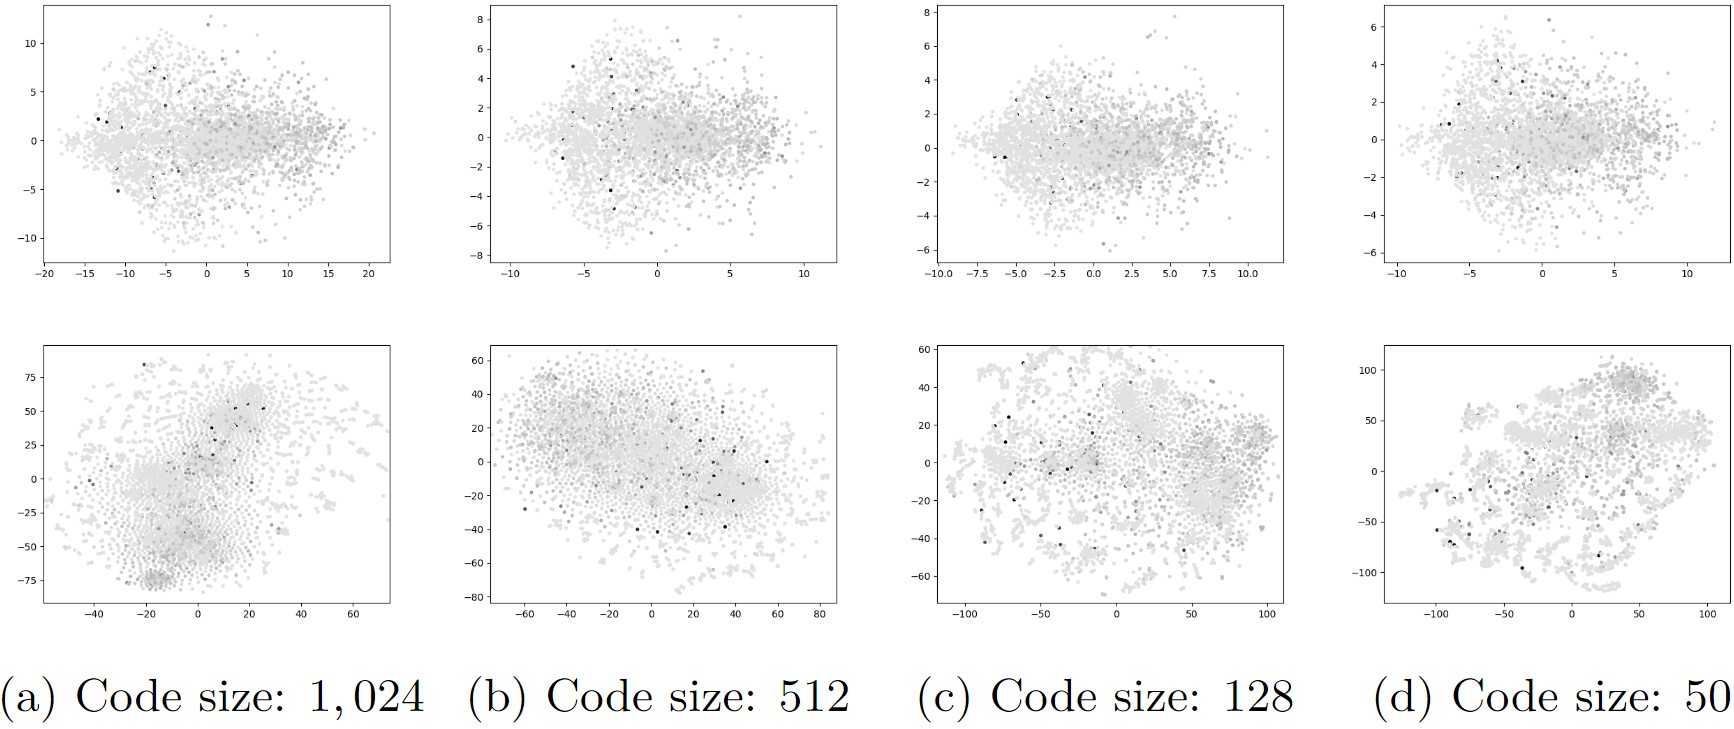
\includegraphics[width=\textwidth]{images/figures/presentation/tsne-DSM.jpg}
	\end{figure}
    \vspace{1.0cm}
\end{frame} 

\section*{15. Ergebnisse: Eingabebilder}
\label{sec:15-images}
\begin{frame}
\frametitle{\begin{center} \Large\bf \nameref{sec:15-images}\end{center}}\vspace{-0.4cm}
    \begin{figure}
		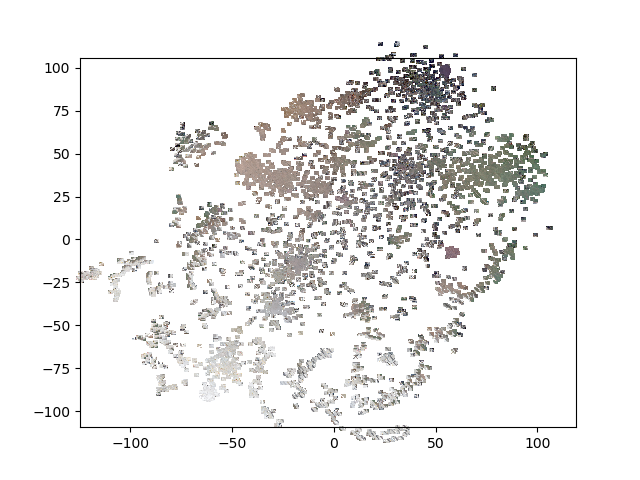
\includegraphics[width=\textwidth]{images/figures/experiments_latent/convolutional_dim50_images.png}
	\end{figure}
    \vspace{1.0cm}
\end{frame} 

\section*{16. Richtungscluster}
\label{sec:16-clusters1}
\begin{frame}
\frametitle{\begin{center} \Large\bf \nameref{sec:16-clusters1}\end{center}}\vspace{-0.4cm}
    \begin{figure}
		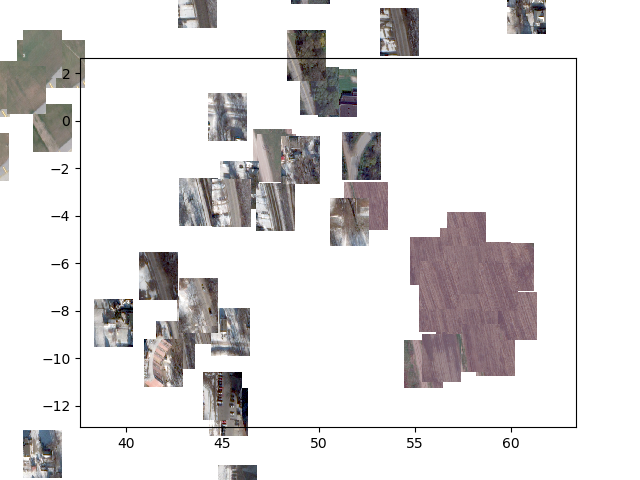
\includegraphics[width=\textwidth]
		{images/figures/experiments_latent/convolutional_dim50_images_upwards_observation.png}
	\end{figure}
    \vspace{1.0cm}
\end{frame} 

\section*{17. Straßencluster}
\label{sec:17-cluster2}
\begin{frame}
\frametitle{\begin{center} \Large\bf \nameref{sec:17-cluster2}\end{center}}\vspace{-0.4cm}
    \begin{figure}
		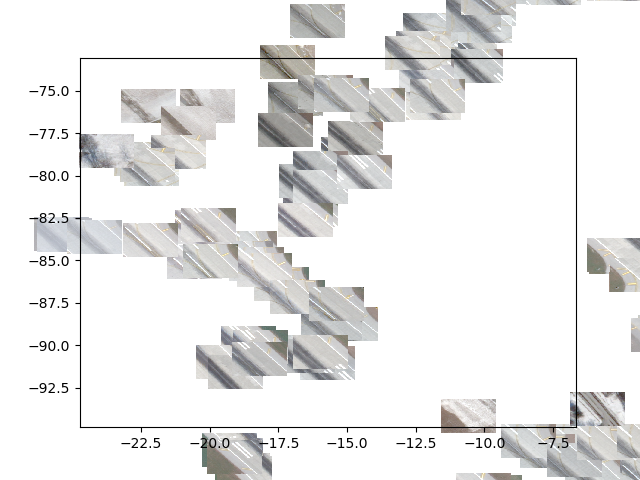
\includegraphics[width=\textwidth]
		{images/figures/experiments_latent/convolutional_dim50_images_sideways_street3.png}
	\end{figure}
    \vspace{1.0cm}
\end{frame}

\section*{18. Fazit und wie es weiter gehen kann}
\label{sec:18-conclusion}
\begin{frame}
\frametitle{\begin{center} \Large\bf \nameref{sec:18-conclusion}\end{center}}\vspace{-0.4cm}
    \begin{itemize}
		\item Der VAE lernt nach komplizierten Features zu clustern
		\item Mit t-SNE kann man die Cluster gut visualisieren
		\item Gute Rekonstruktionen vs. Guter Latenter Raum?
		\item Präzisere Methoden um Cluster zu Features zuzuordnen
		\item Als nächstes bei anderen Tasks als bei Autoencodern testen
	\end{itemize}
    \vspace{1.0cm}
\end{frame}

\section*{19. Rekonstruktionen und Enkodierungsgröße}
\label{sec:19-conclusion}
\begin{frame}
\frametitle{\begin{center} \Large\bf \nameref{sec:19-conclusion}\end{center}}\vspace{-0.4cm}
    \begin{figure}
		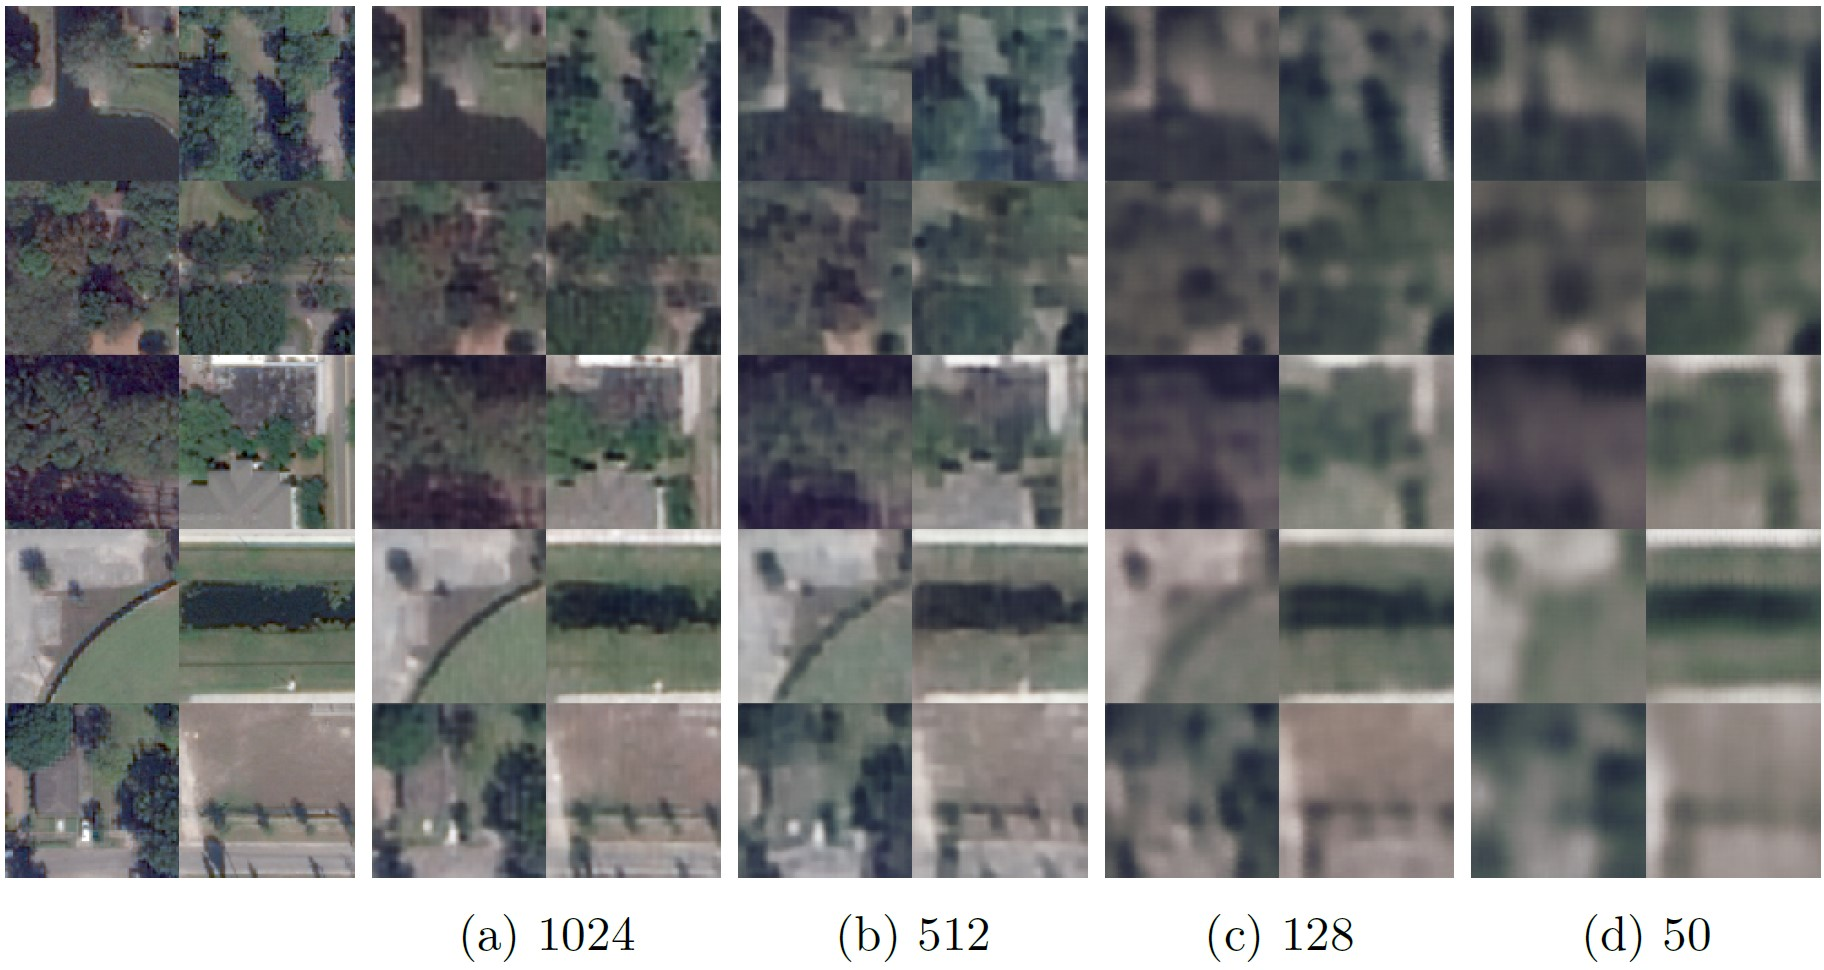
\includegraphics[width=\textwidth]{images/figures/presentation/reconstruction_vs_continuity.jpg}
	\end{figure}
    \vspace{1.0cm}
\end{frame}

